% uidesign.tex

\chapter{User interface elements} \label{chap:uidesign}
C++ does not have a default user interface library. Therefore, the user
interface architecture presented in Section \ref{sect:design:ui_architecture}
needs to be implemented with a special toolkit. This toolkit will supply a set
basic elements that can be extended with custom, specialized elements.

\bigskip \noindent
The main goal of this chapter is to present the user interface elements the
application uses. These are the user interface elements provided by the chosen
toolkit as well as some custom elements.

\bigskip \noindent
The choice for a specific toolkit is made in Section
\ref{sect:uidesign:toolkit}. After that decision has been made, the user
interface elements supported by that toolkit will be described briefly. The
custom user interface elements will then be presented in Section
\ref{sect:uidesign:custom}.

%%%%%%%%%%%%%%%%%%%%%%%%%%%%%%%%%%%%%%%%%%%%%%%%%%%%%%%%%%%%%%%%%%%%%%%%%%%%%
\section{Choosing a user interface toolkit} \label{sect:uidesign:toolkit}
There are several widget toolkits available for all flavors of unix operating
systems. The most popular toolkits that interface directly with C/C++ are
listed below:
\begin{itemize}
\item Motif or Lesstiff
\item The Athena widget library
\item GTK+
\item Qt
\end{itemize}

\bigskip \noindent
\textbf{Motif (or Lesstiff)} is well known. Motif provides a rich set of user
interface elements and is quite powerful. The main disadvantage of Motif is the
old C-style function based interface.


\bigskip \noindent
\textbf{The Athena widget library} is also function based. The Athena widget
set is very easy to learn but (as a consequence perhaps) not as rich as for
example Motif.

\bigskip \noindent
\textbf{GTK+} is used in GNOME. It is a very complete toolkit. Contrary to
Motif and Athena, this toolkit is object oriented. It is also a portable
toolkit, although it has many dependencies that can make compilation difficult.

\bigskip \noindent
\textbf{Qt} is the toolkit on which the KDE window manager is based. Qt
\cite{Qt} is also very complete and object oriented. It was designed with
portability in mind and is available for all Unix platforms as well as for
Windows. There is even a version for embedded devices. It also provides an
extension to C++ with the signal/slot mechanism.

\bigskip \noindent
The choice seems to be between Qt and GTK+. Qt was chosen because of its
portability and the signal/slot mechanism.

%%%%%%%%%%%%%%%%%%%%%%%%%%%%%%%%%%%%%%%%%%%%%%%%%%%%%%%%%%%%%%%%%%%%%%%%%%%%%
\section{Qt native user interface elements}
Qt's complete list of user interface elements is too large to describe here.
The elements that will be described next are the ones that are supported by the
configuration file language as well as those that are used for the custom
widgets. Readers that are already familiar with these widgets can skip to
Section \ref{sect:uidesign:custom}.

\subsection{Labels and edits}
Labels and editable widgets are heavily used. They are implemented by the
\verb=QLabel= and \verb=QLineEdit= classes.

A label is a frame containing text. This text cannot be changed by the user.
Contrary to this, the edit widget \emph{can} be changed by the user. The main
use for this type of widget is to retrieve numbers or text from the user.

Figure \ref{fig:uidesign:label_edit} shows these two widgets in action.

\begin{figure}[ht] \begin{center}
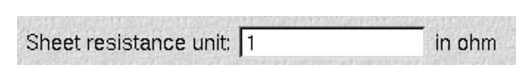
\includegraphics[height=5mm]{./figures/label_edit.eps}
\caption{Two label widgets and one edit widget.}
\label{fig:uidesign:label_edit}
\end{center} \end{figure}

\subsection{Dropdowns and comboboxes}
Dropdowns can be used if the user can choose a value from a list of known
values. A combobox should be used if it must also be possible for the user to
type in a value not found in the list.

For example, suppose the user must enter a month name. In this case, a dropdown
should be used containing the twelve moths of the year. Now suppose the user
must enter a word he would like to search for in a document. It is common
practice to also let the user choose from the last few search terms. In this
case the combobox contains the last few search terms but it is still possible
to enter a new search term.

\bigskip \noindent
Figure \ref{fig:uidesign:combobox} shows a combobox. The widgets are
implemented by the \verb=QComboBox= class. Dropdown behaviour can be achieved
by making the \verb=QComboBox= read only.

\begin{figure}[ht] \begin{center}
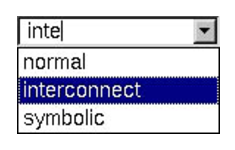
\includegraphics[height=15mm]{./figures/combobox.eps}
\caption{A combobox widget.}
\label{fig:uidesign:combobox}
\end{center} \end{figure}

\subsection{Listview}
The listview widget is often used to display files and their properties. A
screenshot of listview is depicted in Figure \ref{fig:uidesign:listview}.
\begin{figure}[ht] \begin{center}
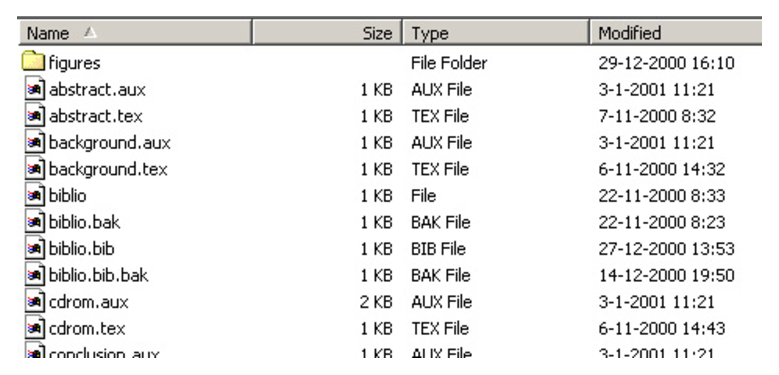
\includegraphics[height=3cm]{./figures/listview.eps}
\caption{A listview widget used to display files.}
\label{fig:uidesign:listview}
\end{center} \end{figure}
Listviews usually have multiple columns. Clicking a row selects the entire row
and editing is limited to the first column, if editing is allowed at all.

\subsection{The color select dialog box}
Color selection is also directly provided by Qt. The \verb=QColorDialog= class
implements a color selection dialog that can be called and used with one line
of code. A screenshot is shown in Figure \ref{fig:uidesign:colordialog}.

\begin{figure}[hb] \begin{center}
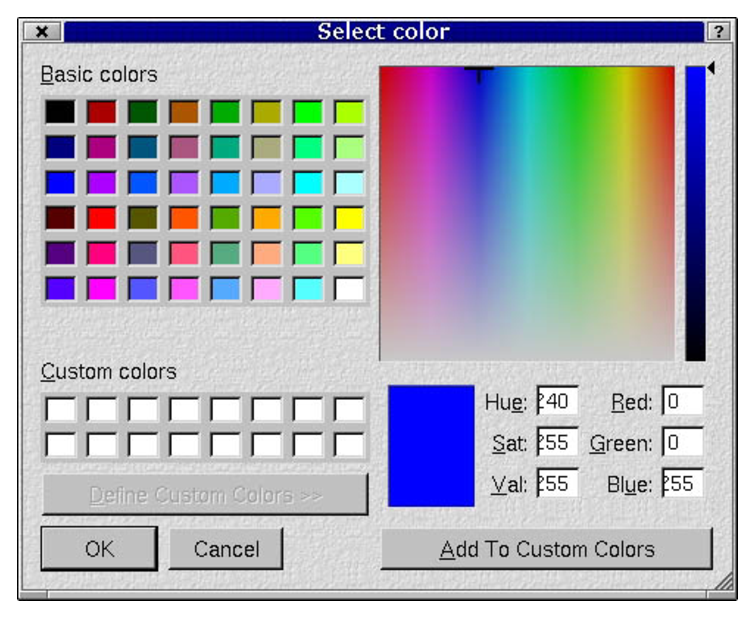
\includegraphics[height=5cm]{./figures/color.eps}
\caption{The Qt color selection dialog box.}
\label{fig:uidesign:colordialog}
\end{center} \end{figure}

%%%%%%%%%%%%%%%%%%%%%%%%%%%%%%%%%%%%%%%%%%%%%%%%%%%%%%%%%%%%%%%%%%%%%%%%%%%%%
\section{Custom user interface elements} \label{sect:uidesign:custom}
Not a single toolkit provides the specialized widgets a programmer always seems
to need. The reason for this is simple: toolkits are designed to be general.
However, extending the toolkit should be easy and with Qt it really is.

The widgets created can be split into two categories:
\begin{enumerate}
\item Organizational widgets.\\ These widgets alter the presentation and layout of the widgets
they contain. These are the scrollframe and the section widget.
\item Data entry widgets.\\ These widgets provide a new way to enter data.
These are the spreadsheet widget, the conditionlist dialog and the dali
colorpicker dialog.
\end{enumerate}

\subsection{The scrollframe widget}
The scrollframe widget is used when a part of the user interface becomes to
large to display on the screen. If this happens, the scrollframe widget will
show horizontal and/or vertical scrollbars that can be used to ``scroll'' the
user interface to show the hidden parts.

The best place for them is inside the tabpages. If the widgets will not fit in
the space the tabpage has available, the scrollbars will be shown.

\subsection{The section widget} \label{sect:uidesign:section}
The section widget is a widget that can show or hide it's contents on the users
request. It is especially useful if used in combination with other section
widgets. Section widgets can be nested if desired. It is recommended to make
them part of a scrollframe, as expanding all the widgets will require a lot of
space.

\begin{figure}[ht] \begin{center}
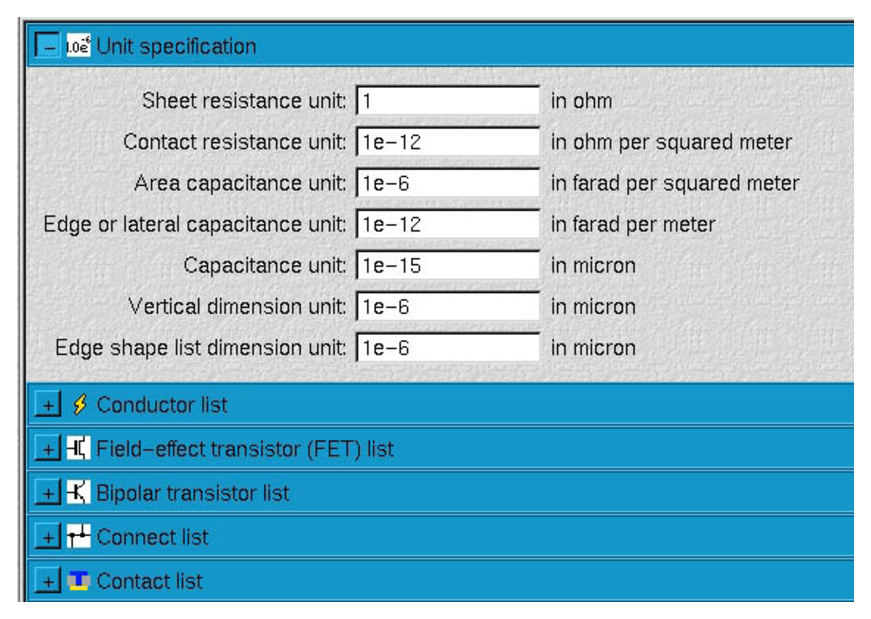
\includegraphics[height=6cm]{./figures/section.eps}
\caption{A few section widgets.}
\label{fig:uidesign:section}
\end{center} \end{figure}

The section widget is demonstrated in Figure \ref{fig:uidesign:section}. The
section widget is a blue bar with a button and a label. It is also possible to
add an icon between the button and the label. If a section is expanded the
button is shown pressed and it will contain a -- sign, indicating it can be
collapsed. If a section is collapsed the button is shown depressed and it will
contain a + sign, indicating it can be expanded.

The section widget has been created to add an extra level of partitioning to
the user interface. This has been discussed in detail in Section
\ref{sect:design:generatedui}.

\subsection{The spreadsheetview widget} \label{sect:uidesign:spreadsheet}
The spreadsheetview widget is a hybrid of a spreadsheet and a listview,
extended with behaviour to make the widget more generally applicable.

\bigskip \noindent
The spreadsheetview visually resembles the listview. However, the default
listview behaviour is not adequate for our purposes. The main deficiencies are
listed below:
\begin{itemize}
\item Editing a cell can only be done with a simple in-place text edit widget.
\item Only the cells in the first column can be edited.
\item Only cells containing text are allowed.
\item The selection and focus behaviour is row oriented and not cell oriented.
\end{itemize}
What we would like to see is a listview in which each cell can be edited. The
way in which a cell can be edited should not be restricted to entering text. It
should be possible to use comboboxes or even dialog boxes to enter a value in a
cell. For example, to specify a layer's color, a cell that can display the
current selected color is necessary. Editing this cell should somehow allow the
user to pick any of the available colors.

The best way to implement this in a flexible way is by using an abstract
\verb=CCell= class. Deriving from this class allows the implementation of
specialized behaviour. There are already five \verb=CCell= derived classes
implementing special cell behaviour. They are listed below:

\begin{itemize}
\item \verb=CEditCell= implements a regular text cell that can be edited with
an in-place line edit.
\item \verb=CComboCell= implements a combobox and dropdown cell. The normal
display is plain text. The edit mode brings up an in-place dropdown or
combobox.
\item \verb=CColorCell= shows a color. The edit mode brings up the default Qt
color select dialog box.
\item \verb=CDaliCell= shows colors and fills as used in dali. The edit mode
brings up the dali colorpicker dialog (which will be described later in this
chapter).
\item \verb=CConditionListCell= shows a conditionlist in the format used in the
SPACE element definition files. The edit mode brings up the conditionlist
editor (which will be described later in this chapter).
\end{itemize}

The spreadsheetview widget is shown in Figure
\ref{fig:uidesign:spreadsheetview}.

\begin{figure}[ht] \begin{center}
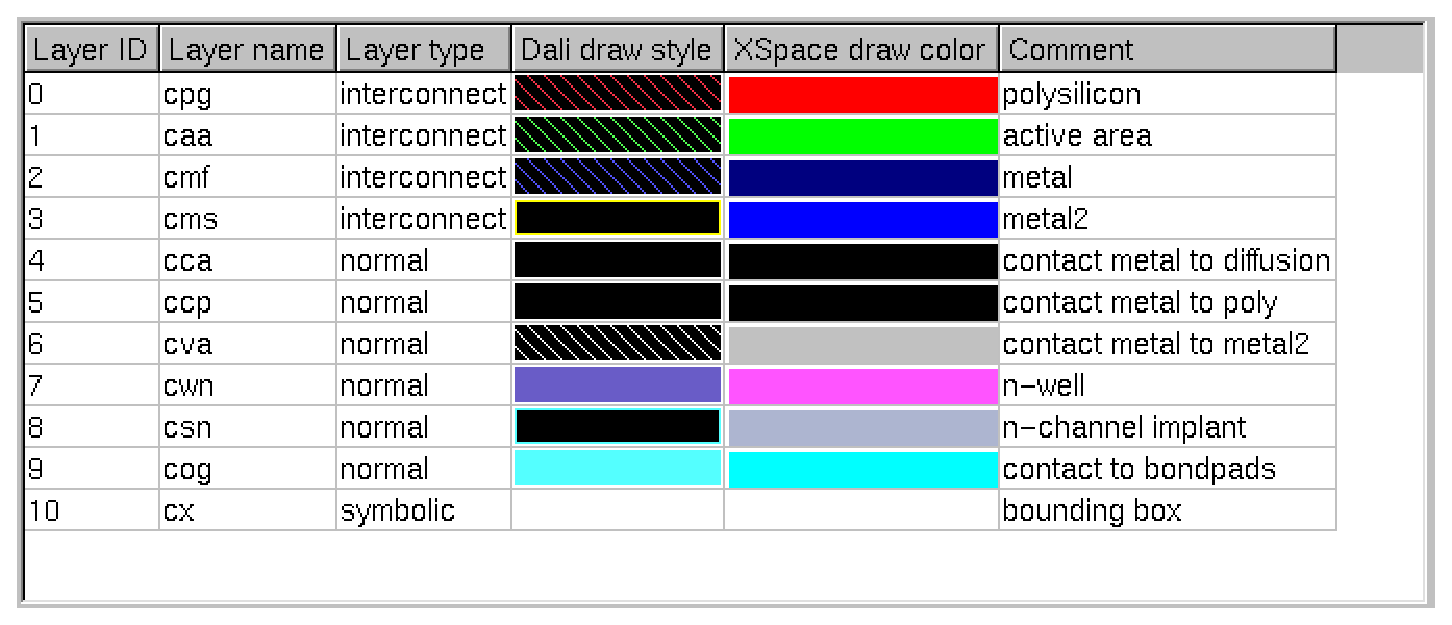
\includegraphics[width=8cm]{./figures/ex_spreadsheet.eps}
\caption{The spreadsheetview widget.}
\label{fig:uidesign:spreadsheetview}
\end{center} \end{figure}


\paragraph{Implementation\\ }
\noindent The spreadsheetview widget is implemented in the
\verb=CSpreadSheetView= class. This class is derived from the Qt
\verb=QListView= class. Also used in the implementation is the custom
\verb=CMultiTypeItem= class which is derived from the \verb=QListViewItem=
class. Finally, the \verb=CCell= class specifies the interface for the derived
classes and provides some basic functionality. The relationship between the
classes is shown in Figure \ref{fig:uidesign:spreadsheet_coll}.
\begin{figure} \begin{center}
\includegraphics[width=10cm]{./figures/class_cspreadsheetview_coll_graph.eps}
\caption{CSpreadSheetView collaboration diagram.}
\label{fig:uidesign:spreadsheet_coll}
\end{center} \end{figure}

The collaboration diagram clearly shows that a \verb=CSpreadSheetView= is a
specialization of the \verb=QListView= class. The \verb=CMultiTypeItem= class
is a specialization of the \verb=QListViewItem= class and represents a row in
the spreadsheetview. The \verb=CMultiTypeItem= itself contains \verb=CCell=
objects, representing the columns in that row.

Figure \ref{fig:uidesign:spreadsheet_class} shows the class diagram. A
\verb=CSpreadSheetView= class contains rows, implemented by the
\verb=CMultiTypeItem= class. Each row consist of a number of \verb=CCell=
derived objects.

\begin{figure} \begin{center}
\includegraphics[width=10cm]{./figures/spreadsheet_class.eps}
\caption{CSpreadSheetView class diagram.}
\label{fig:uidesign:spreadsheet_class}
\end{center} \end{figure}


\bigskip \noindent
After the creation of a \verb=CSpreadSheetView= object, columns can be added
using the \verb=addColumn()= method. Rows can be added using the
\verb=addNewRow()= method. The creation of the \verb=CCell= objects is left to
the client. If a cell object needs to be created the \verb=CSpreadSheetView=
objects emits a \verb=pleaseCreateCell()= signal. The signal communicates the
\verb=CMultiTypeItem= (the row) and the column that needs a \verb=CCell=
(derived) object. If the \verb=CCell= object is not created after the signal
(either because the signal was not connected to a slot or the slot could not
create a object) a default \verb=CCell= will be created by the
\verb=CSpreadSheetView= itself.

This mechanism allows the client to provide its own \verb=CCell= derived
objects at any column/row combination

\bigskip \noindent
Starting and ending the edit mode of a cell is handled by the
\verb=CSpreadSheetView= class, calling the correct \verb=CCell= object methods
as needed. The latest version of Qt now includes a spreadsheet widget (which
was absent during the development of the \verb=CSpreadSheetView= widget). It
uses the same mechanism of cell abstraction and delayed creation. It also uses
start/end edit methods. Perhaps a future version of the \verb=CSpreadSheetView=
widget should be based on this new Qt widget instead of on the \verb=QListView=
widget.

\subsection{The condition list dialog} \label{sect:uidesign:conditionlist}
Condition lists are used often in the SPACE element definition files. A
condition list specifies how the presence of a particular element depends on
the presence or absence of the different masks \cite{SpaceMan}. Basically, it
is a boolean combination of mask names. A space means the AND operation should
be applied. A \verb=|= character corresponds to an OR operation and an
exclamation mark (!) in front of a mask name is a NOT. Additionally, in the
cases where adjacent tiles have a meaning, the -- and = characters specify one
or the other side of a tile. For more information please refer to the SPACE
User's Manual \cite{SpaceMan}.

\begin{figure} \begin{center}
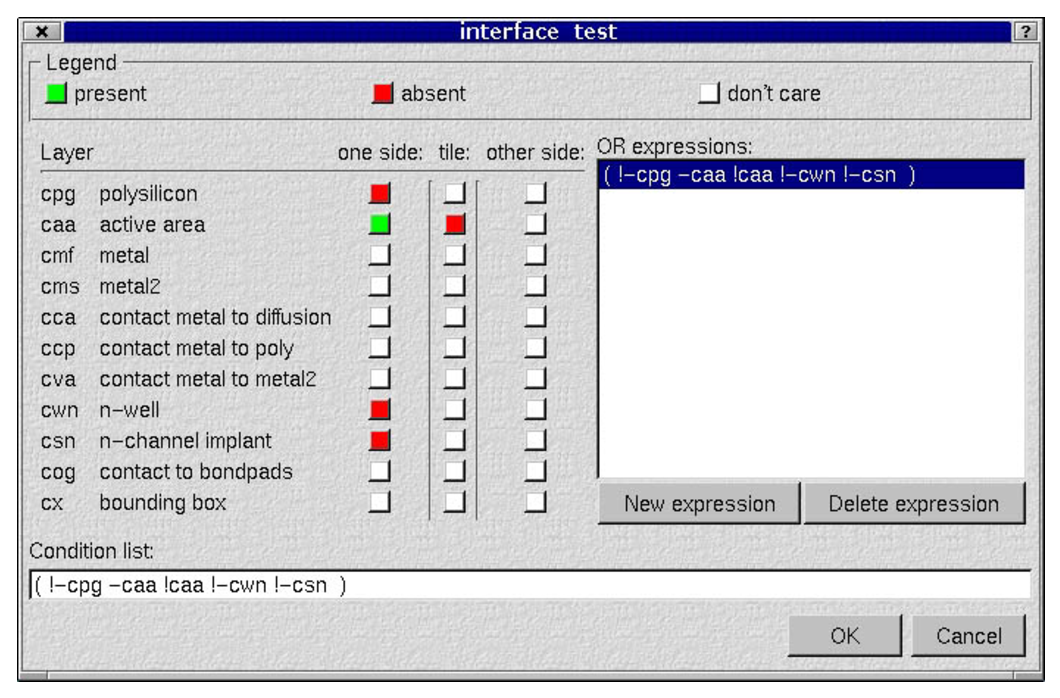
\includegraphics[width=9cm]{./figures/conditionlist.eps}
\caption{The conditionlist editor dialog box.}
\label{fig:uidesign:conditionlist}
\end{center} \end{figure}

\bigskip \noindent
The condition list editor is shown in Figure \ref{fig:uidesign:conditionlist}.
The condition list can be entered manually or by using the buttons and the
listbox. The layer names and descriptions are obtained using the data
connection mechanism described in Section \ref{sect:design:dataconnections}.
The special data target \verb=CConditionListDataTarget= has been implemented
for this to work. This allows to specify arbitrary sources for the layer names
and descriptions in the configuration file.

The listbox on the right side of the dialog box contains the OR expressions.
Each line in the listbox is OR-ed together to form the complete condition list.
Selecting an expression in this listbox will cause the buttons on the left side
to reflect the selected expression. Changing the button states will immediately
update the selected line in the listbox, as well as the line representing the
complete condition list.

\bigskip \noindent
The condition list editor supports two modes. In the default mode, only the
tile of interest is displayed. No neighboring tiles can be selected as present
or absent. In the extended mode, neighboring tiles are displayed as ``one
side'' and ``other side'' and can be selected as normal. The desired mode can
be specified in the configuration file.

\subsection{The dali colorpicker dialog}
The dali colorpicker dialog box lets the user select a color and fill style as
used in dali, the layout editor. Since dali understands only a limited set of
colors and fill patterns, the default Qt color dialog box and fill patterns
could not be used.

The colorpicker presents the user with a dialog box as shown in Figure
\ref{fig:uidesign:dalicolorpicker}. The dialog box consists of an array of
buttons. All the combinations of available colors with available patterns are
present. Clicking a button selects the color and fill represented by the
button.

\begin{figure}[hb] \begin{center}
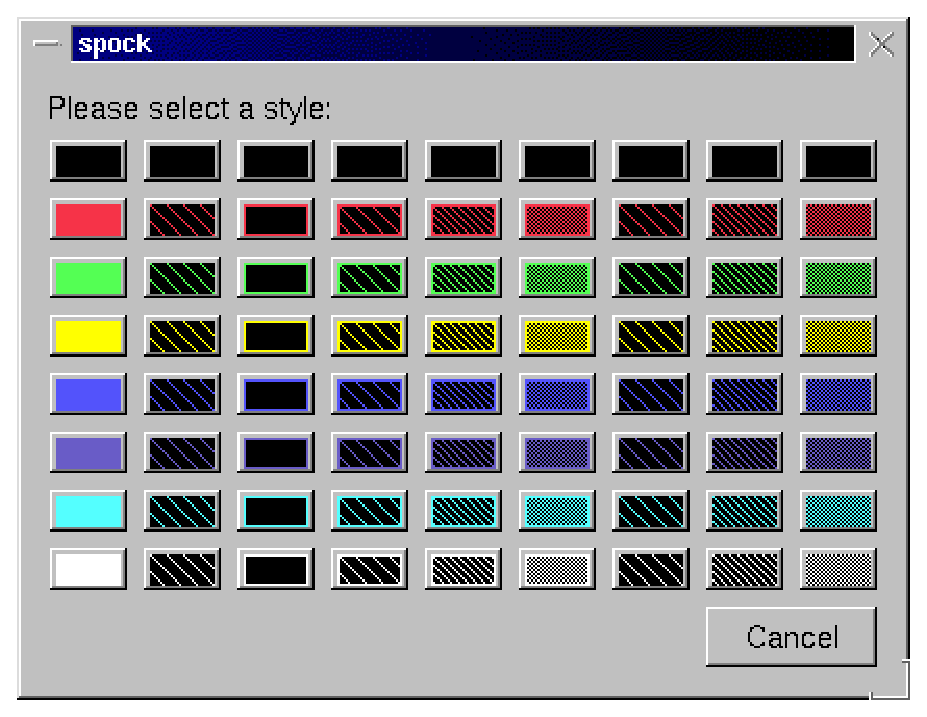
\includegraphics[width=6cm]{./figures/dalicolor.eps}
\caption{The dali colorpicker dialog box.}
\label{fig:uidesign:dalicolorpicker}
\end{center} \end{figure}
